\chapter{Object Detection Using Computer Vision}

\paragraph*{}
Building upon our previous progress report, this section describes the use of the S3 RPLiDAR in conjunction with a webcam for detecting object width, estimating relative distance, and determining angular position of objects. The initial objective was to develop a model capable of detecting and analyzing three cylindrical objects—tested one at a time—since only one cylinder would be present in the arena at any given moment alongside three mobile robots. However, this setup was later refined: the number of cylinders used in the real-world environment was reduced to two—a blue cylinder (16~cm diameter) and a yellow cylinder (20~cm diameter). A third cylinder with a 12~cm diameter was reserved for testing the model's flexibility and generalization.

\paragraph*{}
To summarize the detection pipeline: the robot moves randomly until a target cylinder is detected. Detection is considered valid when the center of the bounding box falls between pixel positions 600 and 680, assuming 0 is the leftmost pixel. Once this criterion is met, a bounding box is drawn, the system state is set to \texttt{FoundObject}, and the robot halts for three seconds. During this pause, the system calculates the relative distance (from the robot’s center to the object surface at the bounding box center), the relative angle, and the estimated diameter. The workflow is illustrated in Figure~\ref{fig:workflow}.

\begin{figure}[H]
    \centering
    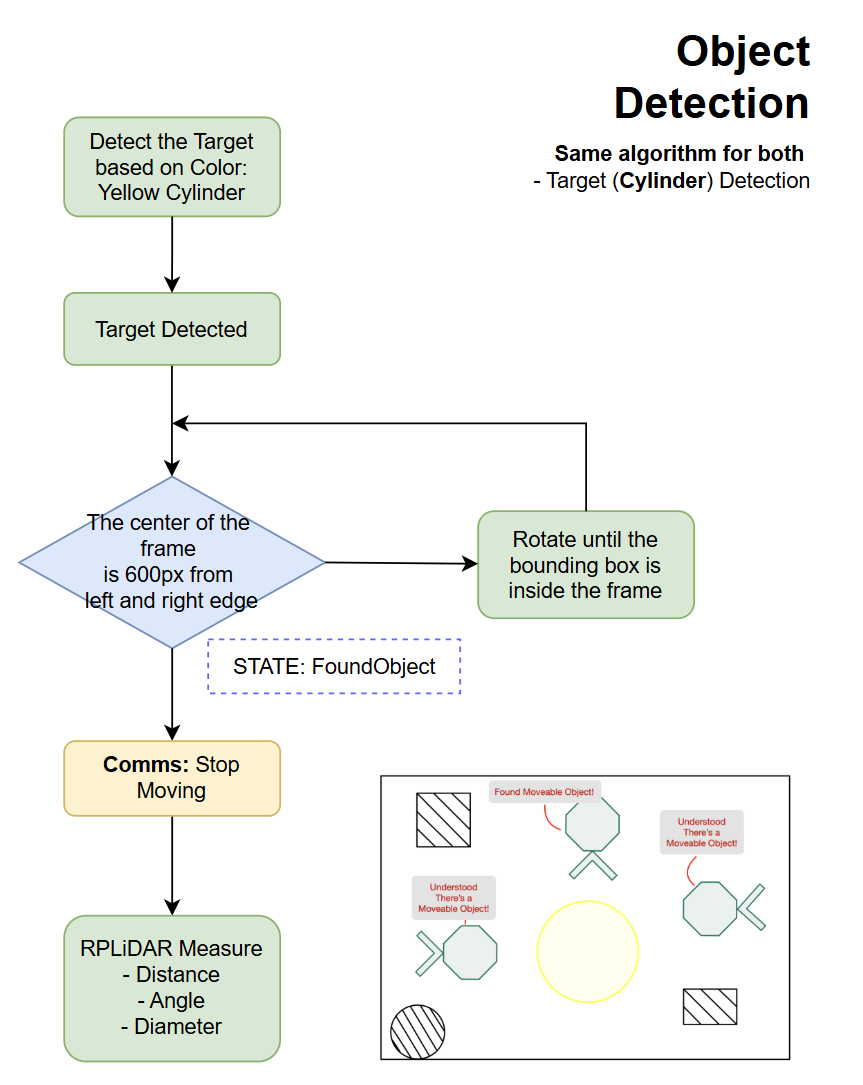
\includegraphics[width=0.5\textwidth]{assets/images/object_detection/fig1.png}
    \caption{Overview of the object detection and measurement workflow}
    \label{fig:workflow}
\end{figure}

\paragraph*{}
Object detection is performed using color segmentation based on the YCbCr color space. Only two colors—blue and yellow—were tested, each defined by specific value ranges within the YCbCr space. The range for blue is [0, 100, 140] to [255, 255, 255], and yellow is [100, 140, 50] to [255, 255, 100].

\paragraph*{}
To enable accurate measurement and computation, multi-sensor fusion is implemented. A key factor in this process is the horizontal field of view (FoV) of the camera, determined through calibration using OpenCV. The calibration process uses images of a checkerboard pattern to estimate the camera’s intrinsic parameters. The horizontal FoV was calculated to be 72 degrees.

Mapping the object’s angular position from the camera frame to the LiDAR frame is achieved using the equation:

\begin{equation}
\text{relative\_angle} = \left( \frac{\text{object\_center\_x} - \text{frame\_center\_x}}{\text{frame\_width}} \right) \times \text{horizontal\_fov}
\label{eq:relative_angle}
\end{equation}

\paragraph*{}
Once the relative angle is computed, the LiDAR provides the corresponding angle and distance values, using data retrieved via the \texttt{rclpy} library in ROS 2.

\paragraph*{}
With the relative distance and angle known, the cylinder’s diameter is estimated using an image projection method, shown in Figure~\ref{fig:projection_diagram}.

\begin{figure}[H]
    \centering
    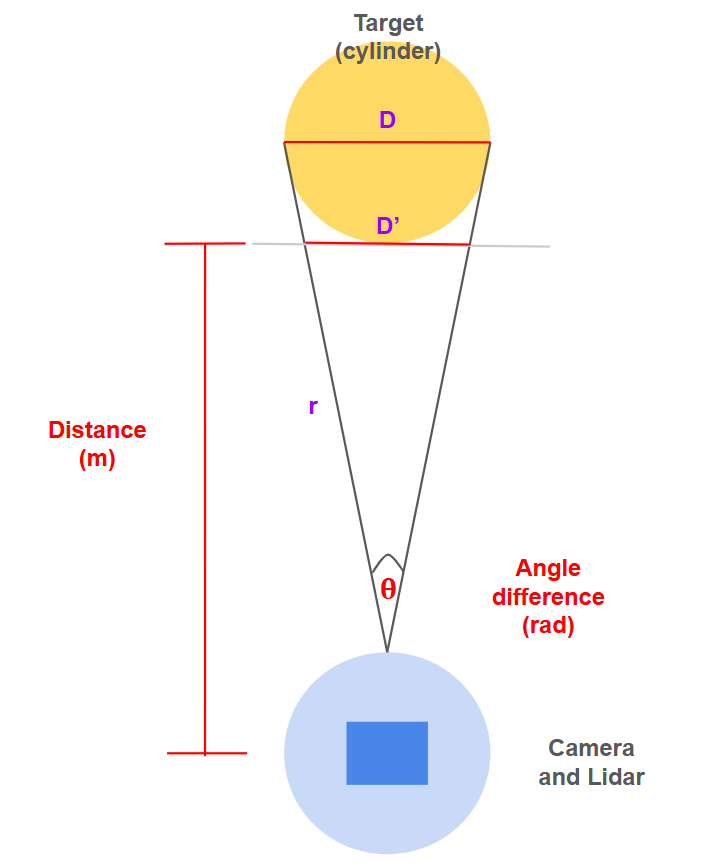
\includegraphics[width=0.5\textwidth]{assets/images/object_detection/fig2.png}
    \caption{Image projection visualization}
    \label{fig:projection_diagram}
\end{figure}

\paragraph*{}
The estimation begins by calculating the distance \( r \) from the LiDAR to the object’s side using:

\begin{equation}
r = \frac{\text{distance}}{\cos\left(\frac{\theta}{2}\right)}
\label{eq:r}
\end{equation}

\paragraph*{}
Here, \( \theta \) is the angle subtended by the object in the camera frame. Then, the projected diameter \( D' \) is computed using the law of cosines:

\begin{equation}
D' = \sqrt{2r^2 - 2r^2 \cos(\theta)}
\label{eq:Dprime}
\end{equation}

\paragraph*{}
The projected radius is:

\begin{equation}
w' = \frac{D'}{2}
\label{eq:wprime}
\end{equation}

\paragraph*{}
Using geometric similarity, the actual radius \( w \) is calculated as:

\begin{equation}
w = \frac{ \text{distance} \cdot \tan\left(\frac{\theta}{2}\right) }{ 1 - \tan\left(\frac{\theta}{2}\right) }
\label{eq:radius_projection}
\end{equation}

\begin{figure}[H]
    \centering
    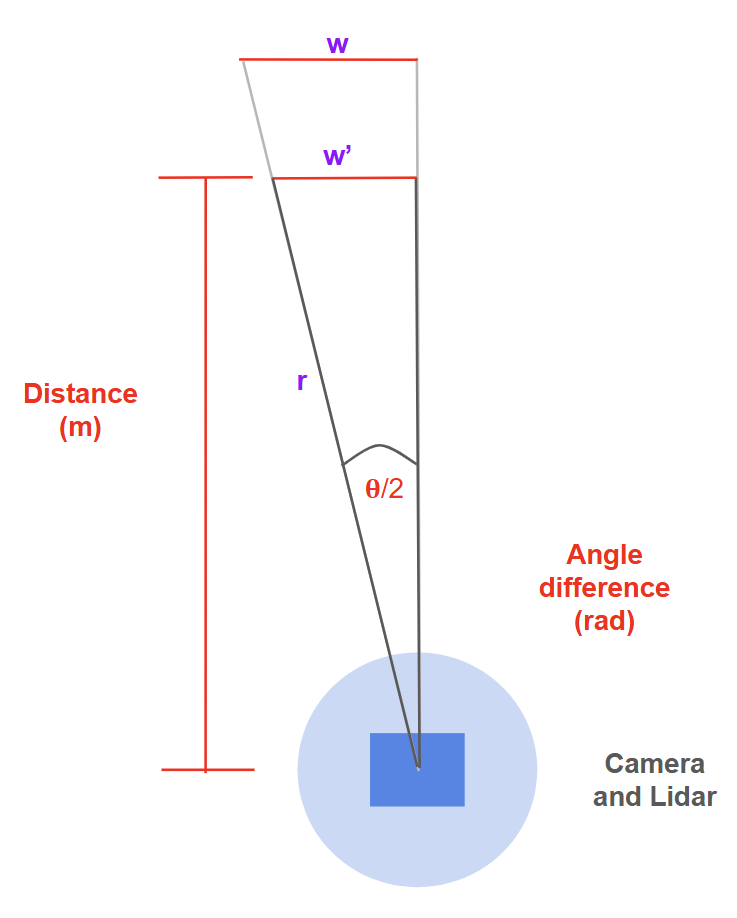
\includegraphics[width=0.5\textwidth]{assets/images/object_detection/fig3.png}
    \caption{Calculation of radius from projected image}
    \label{fig:find_d}
\end{figure}

\paragraph*{}
Although the diameter \( D \) is calculated, camera distortion introduces an error of approximately ±4~cm for distances ranging from 0.4 to 3.0~m. This justifies the constraint on the detection zone to maintain real-world angular accuracy. The calculated diameters are compared against actual measurements in Figure~\ref{fig:D_vs_width}. The model achieved a Mean Absolute Error (MAE) of 0.01289, Mean Squared Error (MSE) of \(2.902 \times 10^{-4}\), and R-squared of 0.0431.

\begin{figure}[H]
    \centering
    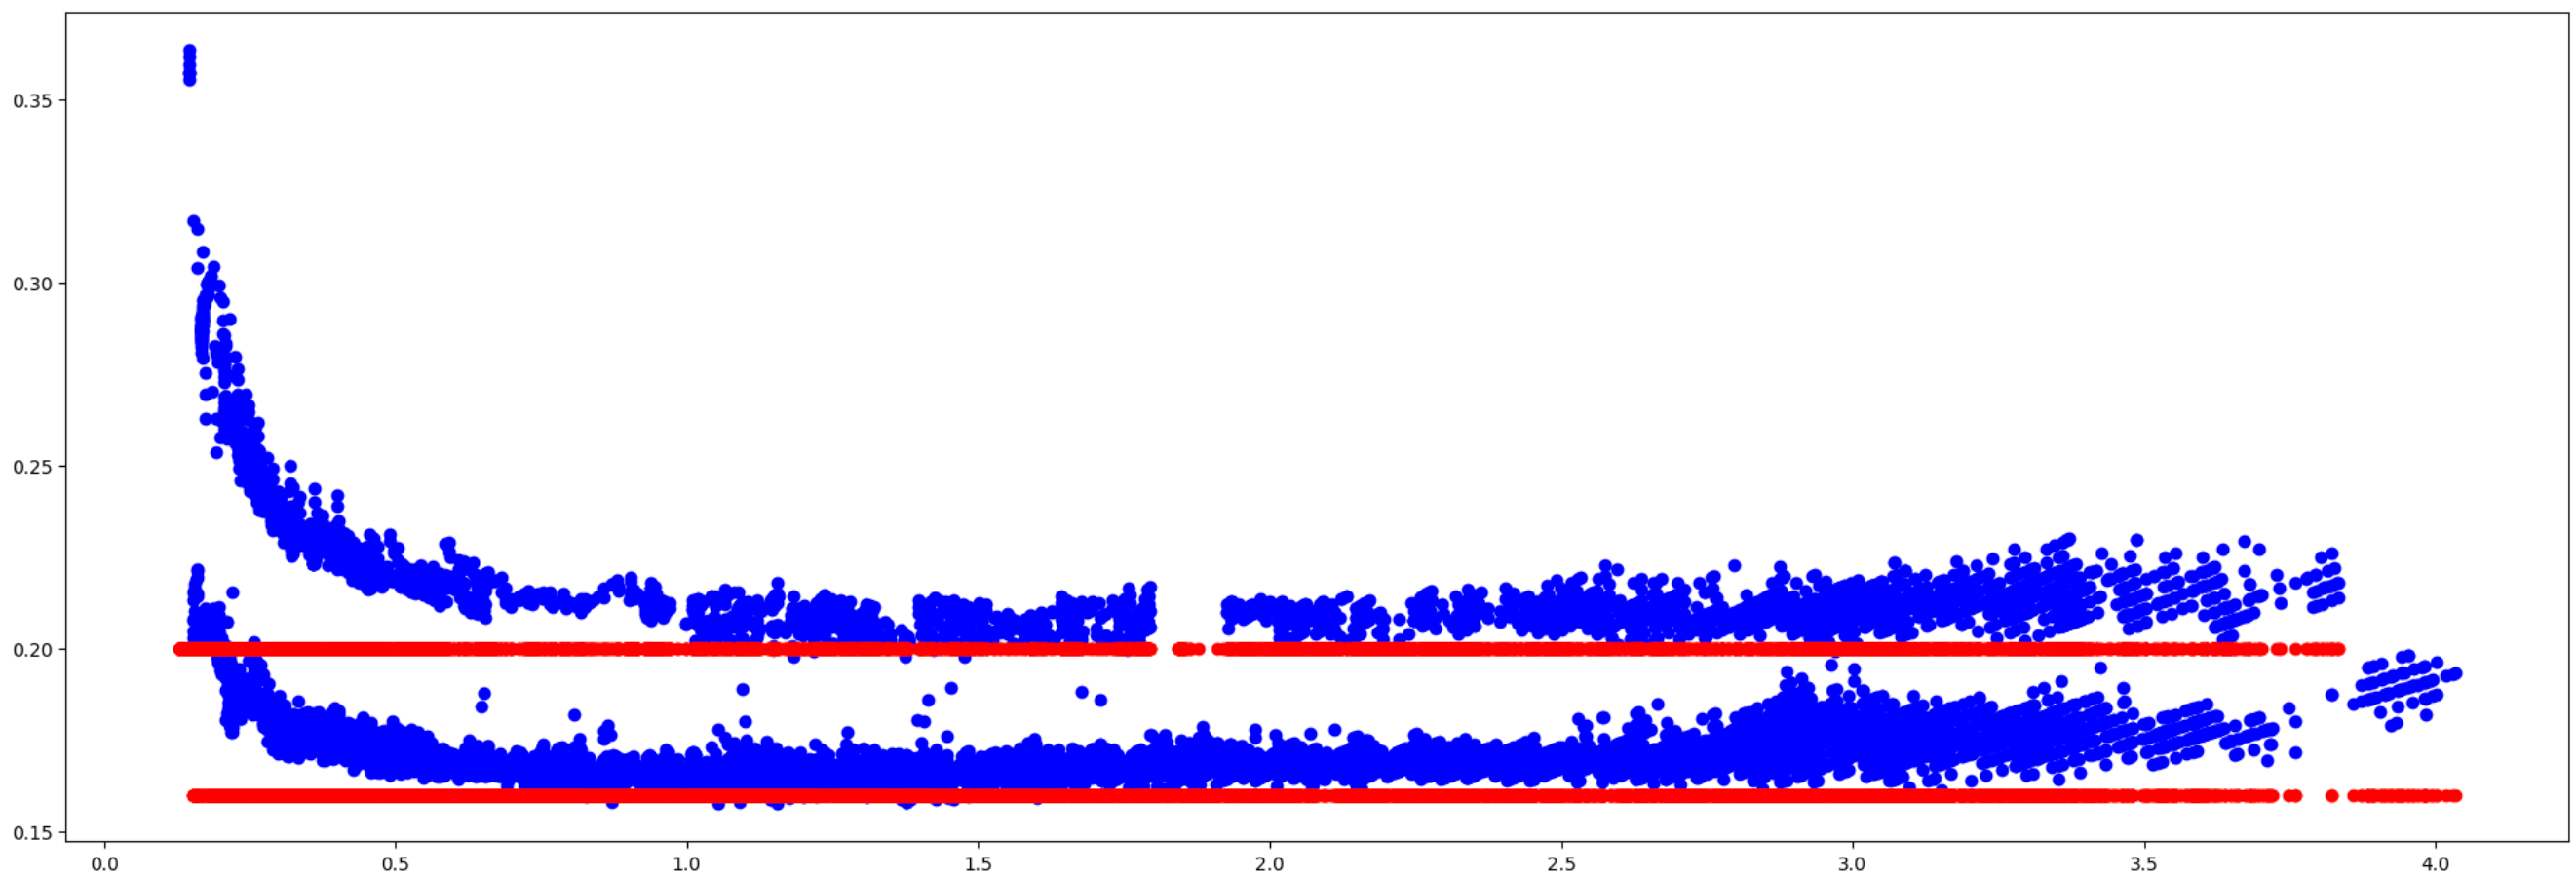
\includegraphics[width=0.9\textwidth]{assets/images/object_detection/fig8.png}
    \caption{Comparison of calculated (blue) vs actual (red) diameters}
    \label{fig:D_vs_width}
\end{figure}

\paragraph*{}
To minimize diameter estimation error, a variation factor is introduced:

\begin{equation}
w' = \frac{\text{actual\_width}}{D}
\label{eq:calculate variation factor}
\end{equation}

\paragraph*{}
The variation factor is computed for each actual-estimated diameter pair. These values are used to train a predictive model using \texttt{scikit-learn}, with distance as the independent variable. 80\% of the dataset is used for training and 20\% for testing. A sigmoid function is fitted to model the relationship, as shown in Figure~\ref{fig:sigmoid}.

\begin{figure}[H]
    \centering
    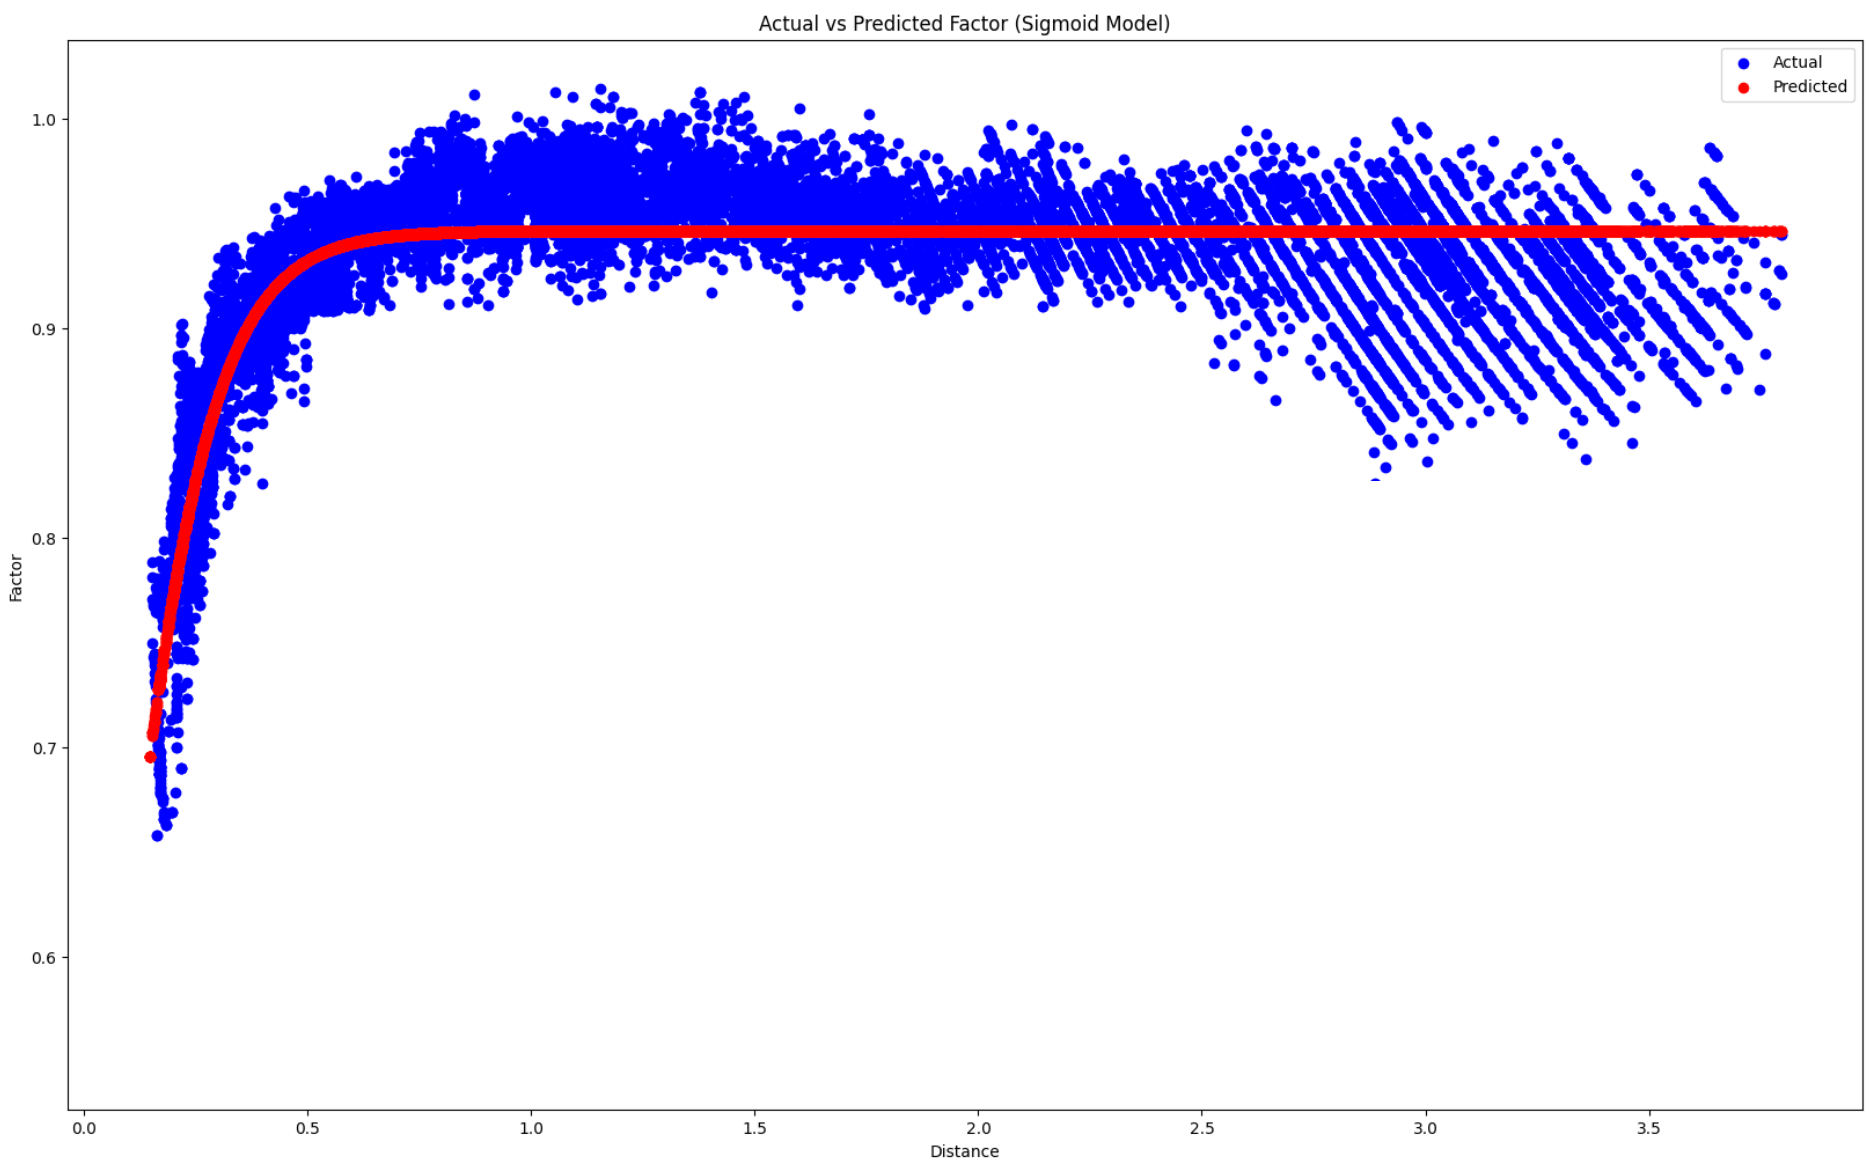
\includegraphics[width=0.9\textwidth]{assets/images/object_detection/fig4.png}
    \caption{Fitted sigmoid function for variation factor}
    \label{fig:sigmoid}
\end{figure}

\paragraph*{}
The final form of the fitted sigmoid function is:

\begin{equation}
\text{factor} = \frac{0.9461218686}{1 + e^{-9.0309891171(x - 0.0335094048)}}
\label{eq:fitted sigmoid}
\end{equation}

\paragraph*{}
Model performance on the test set is evaluated using the following metrics:

\begin{table}[h]
\centering
\caption{Model Accuracy Metrics}
\label{tab:model_accuracy}
\begin{tabular}{|c|c|}
\hline
\textbf{Metric} & \textbf{Value} \\
\hline
Mean Squared Error (MSE) & \(2.802 \times 10^{-5}\) \\
Mean Absolute Error (MAE) & 0.004 \\
R-squared (\(R^2\)) & 0.916 \\
\hline
\end{tabular}
\end{table}

\paragraph*{}
The final cylinder diameter is obtained by multiplying the variation factor by the value of \( D \). The prediction accuracy is visualized in Figure~\ref{fig:width_result}.

\begin{figure}[H]
    \centering
    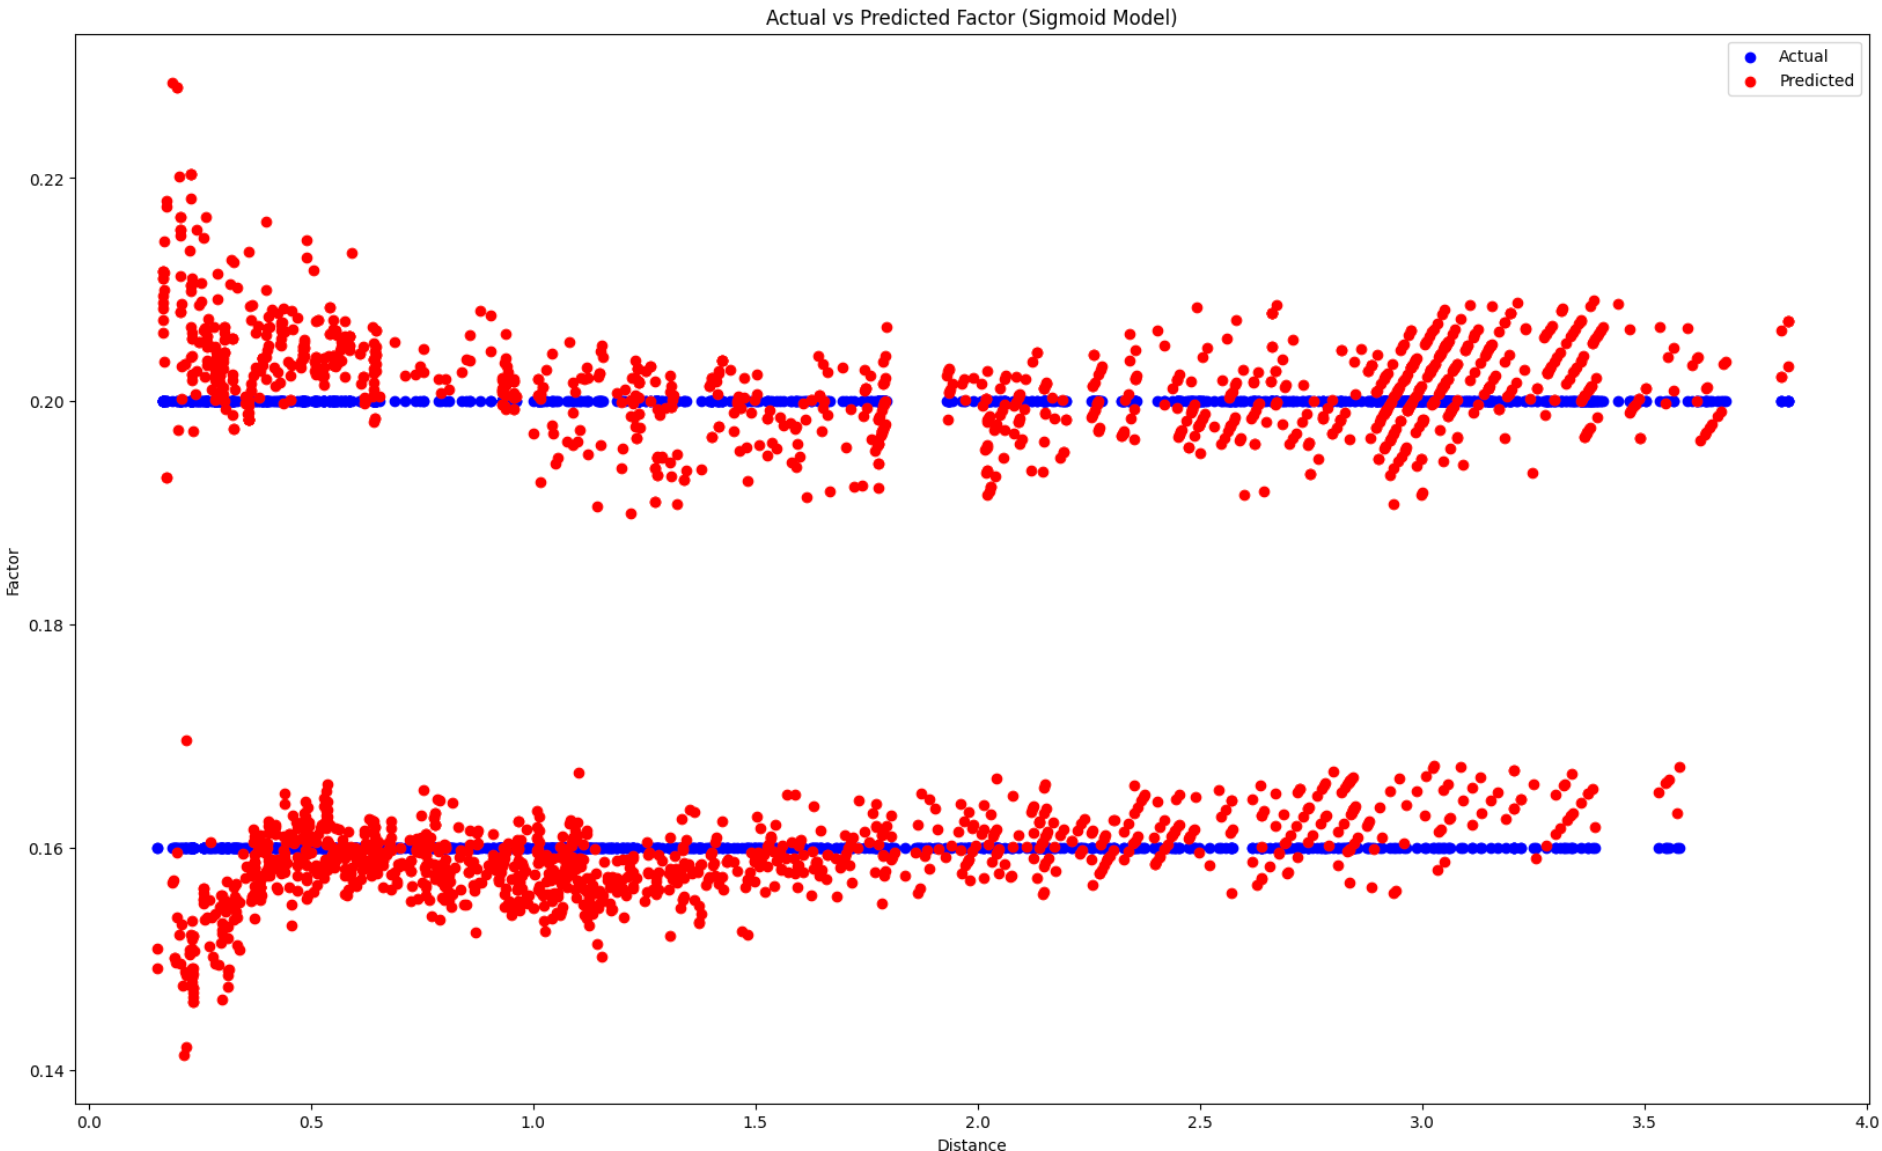
\includegraphics[width=0.8\textwidth]{assets/images/object_detection/fig5.png}
    \caption{Predicted vs actual cylinder diameter}
    \label{fig:width_result}
\end{figure}

\paragraph*{}
Model robustness was evaluated by placing cylinders at distances of 0.5~m, 1~m, 2~m, and 3~m under nine different lighting conditions, shown in Figure~\ref{fig:ligthing conditions}. Lighting conditions 1–8 involved radial illumination at 0.4~m and a 30-degree elevation angle. Condition 9 featured overhead lighting from a height of 0.3~m. All tests were conducted in a darkened lab environment.

\begin{figure}[H]
    \centering
    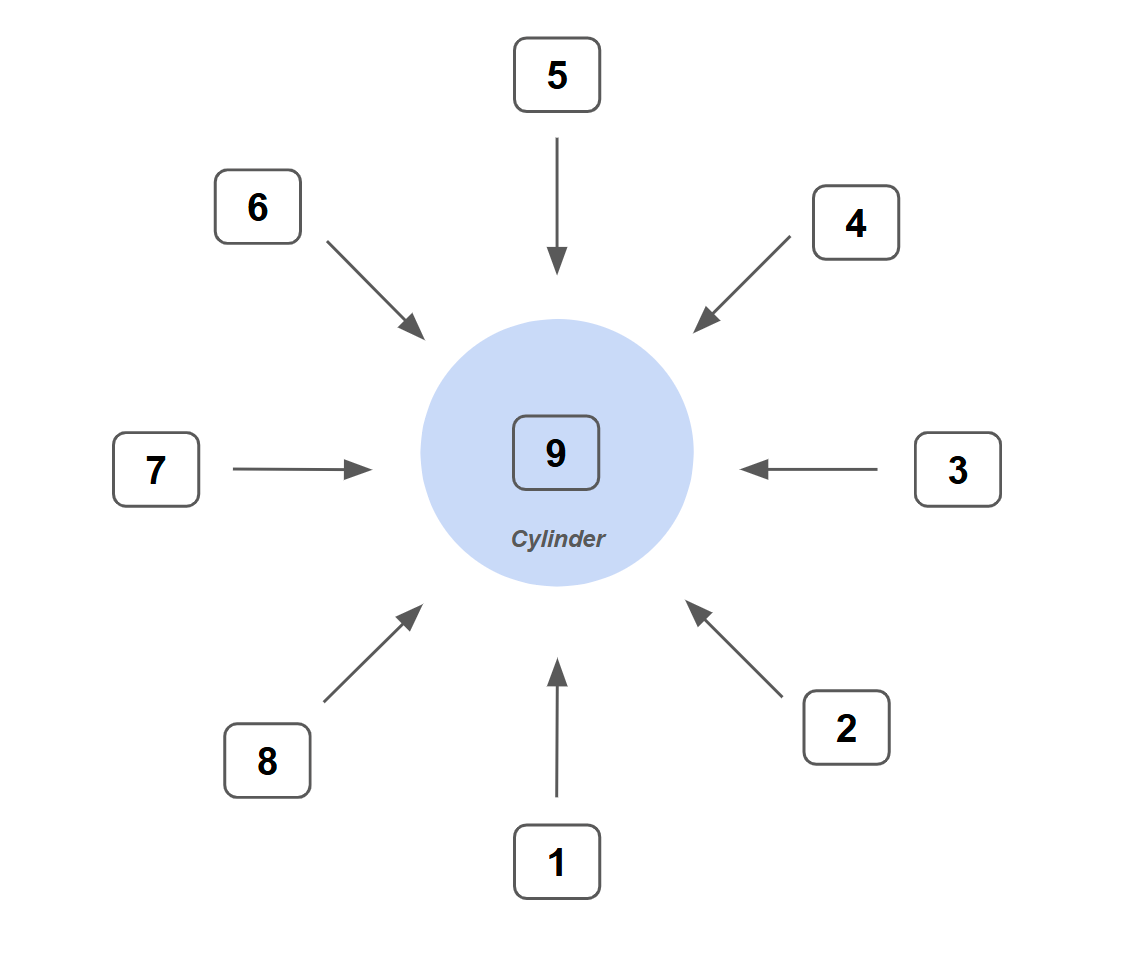
\includegraphics[width=0.7\textwidth]{assets/images/object_detection/fig6.png}
    \caption{Nine lighting conditions used for model testing}
    \label{fig:ligthing conditions}
\end{figure}

\paragraph*{}
Measurements for each cylinder under all lighting conditions are presented in Appendix A. Tables~\ref{tab:20cm} and \ref{tab:16cm} show predicted diameters, relative distances, and angles for the 20~cm and 16~cm cylinders, respectively. Table~\ref{tab:12cm} evaluates the model’s generalization on the 12~cm cylinder. Summary errors are shown in Table~\ref{tab:mean_errors}.

\begin{table}[ht]
    \centering
    
    \label{tab:mean_errors}
    \begin{tabular}{|l|c|c|}
        \hline
        \textbf{Table} & \textbf{Mean Absolute Width Error (m)} & \textbf{Mean Absolute Angle Error (°)} \\
        \hline
        Table 1 & 0.0022 & 0.2389 \\
        Table 2 & 0.0017 & 0.2219 \\
        Table 3 & 0.0061 & 1.0519 \\
        \hline
    \end{tabular}
    \caption{Mean absolute width and angle errors}
\end{table}

\paragraph*{}
After applying a variation factor to optimize the accuracy of width measurements, the model's performance improved significantly. The prediction error was reduced from 4 centimeters to approximately 1 centimeter for cylinders with diameters of 20 cm and 16 cm, which are the objects intended for use in the actual test environment. In contrast, the 12 cm diameter cylinder exhibited a higher prediction error of up to 2 centimeters.

\paragraph*{}
To further enhance the model's flexibility and accuracy, it is recommended to incorporate data from the 12 cm cylinder into the determination of the variation factor function. Ultimately, to generalize the model for different cylinder sizes or even other geometric shapes, the variation factor should be defined as a function of intrinsic and extrinsic camera parameters, which can be accurately obtained through OpenCV camera calibration.
